\documentclass{article}
\usepackage[preprint,nonatbib]{neurips_2026}
\usepackage[T1]{fontenc}
\usepackage{booktabs,graphicx,amsmath,amssymb,hyperref}
\hypersetup{colorlinks=true,linkcolor=blue,urlcolor=blue,citecolor=blue}
\makeatletter\renewcommand{\@noticestring}{ECE661 Team 3 course project, Fall 2026. Course report; not a NeurIPS publication.}\makeatother
\title{Universal Adversarial Patches on CIFAR-10:\\Transferability and Adaptive Defense Evaluation}
\author{Xitai Yu (xy195) \And Russo Zhang (yz1047) \AND Boyi Zhao (bz138) \And Zijiang Yang (zy232)}
\begin{document}\maketitle
\begin{abstract}
We evaluate universal CIFAR-10 patches on three fixed classifiers: 561 main optimizations, 24 strength checks, three patch seeds, and 1,638 audited test conditions. Matched occlusion, EOT-matched defense controls, held-out isolation, and step/time comparisons distinguish texture, attacker knowledge, and computational effects. Reported metrics are recomputed from archived per-image predictions.
ResNet untargeted ASR rises from 8.66\% (side 3) to 89.79\% (side 16). The side-7 ensemble changes held-out targeted macro ASR by -0.10 percentage points at fixed steps and -0.67 at matched time. These digital measurements provide no certified or physical robustness guarantee.
\end{abstract}
\section{Introduction and related work}
Universal patches share a learned texture across images and transformations~\cite{brown}. Defense evaluation must include the complete pipeline, since weak optimization can make preprocessing appear robust~\cite{athalye}. We contribute a controlled comparison at original CIFAR resolution, with matched controls, held-out isolation, computational accounting, and explicit statistical units; ensemble optimization and EOT are existing methods.
\section{A: Data, models, and shared evaluation}
The official CIFAR-10 Python archive passes its published MD5. PCG64(661) selects 500 validation images per class from the 50,000 training images, leaving 45,000 training images. PCG64(662) independently selects 100 validation images per class for patch selection. Channel means and population standard deviations use training pixels only. The untouched 10,000-image test set is evaluated after artifact freezing. All networks consume raw float32 RGB through one internal normalization layer.
\begin{center}\small
\begin{tabular}{lrrr}\toprule
Model & Parameters & Best val. (\%) & Test clean (\%)\\\midrule
ResNet-20 & 269,722 & 92.78 & 92.29\\
VGG-11-BN-CIFAR & 9,756,426 & 92.38 & 91.99\\
DenseNet-BC-40-12 & 176,122 & 92.56 & 92.36\\
\bottomrule\end{tabular}\end{center}
All three classifiers use the exact CIFAR architectures in the research protocol, including Option A ResNet shortcuts and the specified VGG head~\cite{resnet,vgg,densenet}. Supervised training uses 200 epochs, SGD, batch 128, momentum 0.9, weight decay $5\cdot10^{-4}$, initial learning rate 0.1, and cosine decay. Checkpoints maximize full validation accuracy, with earliest ties. Selected patches also receive full 5,000-image source-only validation before freezing (1,212 conditions), without changing selection or querying DenseNet attacks. One classifier training seed (17) is used; patch repeats do not measure classifier-training uncertainty.
\clearpage
\section{B: Universal patches and baseline experiments}
For each side $s\in\{3,5,7,16\}$, objective, and seed 101/102/103, one tensor $p\in[0,1]^{3\times s\times s}$ is shared across all training images. The frozen networks remain in evaluation mode. Each update samples rotation in $[-15,15]$ degrees, scale in $[0.9,1.1]$, and a legal, fully contained location. Premultiplied alpha compositing preserves the background and avoids dark interpolation boundaries. Targeted and untargeted objectives are respectively
\[
\min_p\;\mathbb E\,\mathrm{CE}(f(A(p,x,\tau)),t),\qquad
\min_p\;-\mathbb E\,\mathrm{CE}(f(A(p,x,\tau)),y).
\]
Adam uses learning rate 0.05, batch 128, and 1,000 updates. Step 0 and every 100 updates are validated on the fixed 1,000-image subset with eight draws per image; earliest maximum validation ASR selects the patch. The finite development candidates are learning rates 0.01/0.05 and budgets 500/1,000, for the prespecified 7-by-7 untargeted and target-3 tasks. These development outcomes are separate from test results.
\begin{center}\small
\begin{tabular}{rrrr}\toprule
Side & Nominal area (\%) & UASR (\%) & Target macro TASR (\%)\\\midrule
3 & 0.879 & 8.66 $\pm$ 1.01 & 1.48 $\pm$ 0.13\\
5 & 2.441 & 25.80 $\pm$ 1.55 & 6.24 $\pm$ 1.37\\
7 & 4.785 & 46.56 $\pm$ 1.69 & 24.97 $\pm$ 0.52\\
16 & 25.000 & 89.79 $\pm$ 0.04 & 99.92 $\pm$ 0.01\\
\bottomrule\end{tabular}\end{center}


\begin{figure}[h]
\centering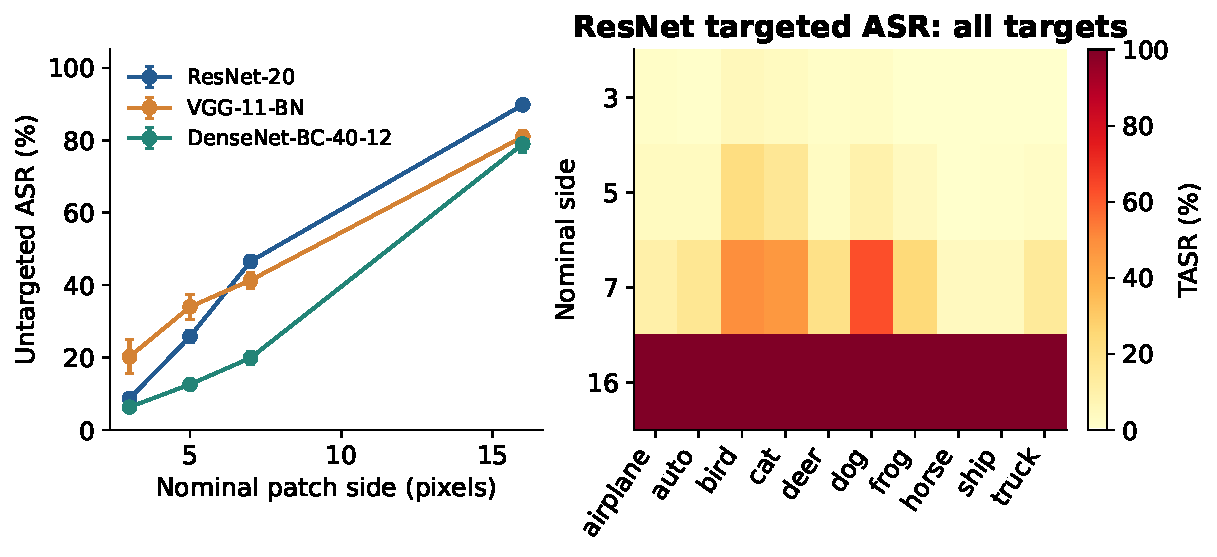
\includegraphics[width=\linewidth,height=2.55in,keepaspectratio]{images/B_size_and_targets.pdf}
\caption{Left: the same ResNet-optimized patches evaluated on each classifier. Right: all ten ResNet target classes, averaging three patch seeds. Error bars are sample standard deviations over patch seeds. Cross-model ASR has model-specific eligibility sets.}
\end{figure}

For the 16-by-16 ResNet condition, optimized untargeted ASR is 89.79\%, compared with 43.70\% for random texture and 44.56\% for mean-color occlusion. These matched controls separate the texture contribution from the effect of removing a quarter of the nominal image area. Effective alpha and support areas are retained in every raw record; transformed coverage is not equated with nominal area. All target classes and all seeds remain in the tables, including weak attacks.
\clearpage
\section{C: Held-out transfer and compute budgets}
The basic 132 ResNet patches transfer without alteration to VGG and DenseNet. The extension compares ResNet (R), VGG (V), and an equal-weight average of their cross-entropy losses (RV). The same rendered images feed both source networks. Averaging losses is distinct from averaging logits. DenseNet provides neither gradients nor attack-selection feedback. Fixed-step comparisons cover sides 5/7 and all eleven objectives, reusing the R patches from B.
For the 7-by-7 time comparison, three 50-update ensemble measurements after independent warmup set a common training budget of 12.833 seconds. Every strategy starts from the paired initialization, checks elapsed time every ten updates, and saves the final budget-ending candidate as well as periodic candidates. Validation pauses this timer; validation, warmup, and end-to-end costs are recorded separately. Faster methods may perform more updates. Time budgets are calibrated on the same RTX 5080 after classifier training ends.
Observed strategy means are R: 1290 updates / 12.885 s, V: 1479 updates / 12.882 s, RV: 907 updates / 12.891 s. Across all 99 runs, training time ranges from 12.834 to 12.992 seconds.


\begin{figure}[h]
\centering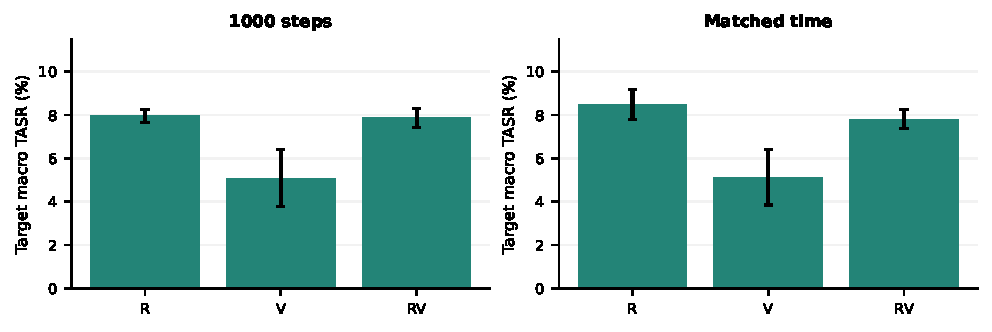
\includegraphics[width=\linewidth,height=2.1in,keepaspectratio]{images/C_main_report.pdf}
\caption{Held-out DenseNet targeted macro ASR for side 7. R and V are single-source optimizers; RV averages their losses. The two panels use distinct budget definitions. Error bars use three independent patch seeds; the table also includes untargeted effects and side 5.}
\end{figure}

\begin{center}\small
\begin{tabular}{lrlrr}\toprule
Budget & Side & Metric & RV - R: pp [95\% CI] & RV - V: pp [95\% CI]\\\midrule
steps & 5 & U & -0.84 [-0.97, -0.71] & -0.13 [-0.21, -0.05]\\
steps & 5 & T macro & -0.30 [-0.32, -0.27] & +0.51 [+0.48, +0.53]\\
steps & 7 & U & -1.43 [-1.62, -1.23] & +3.08 [+2.95, +3.22]\\
steps & 7 & T macro & -0.10 [-0.15, -0.06] & +2.78 [+2.72, +2.85]\\
time & 7 & U & -2.47 [-2.65, -2.27] & +2.57 [+2.43, +2.70]\\
time & 7 & T macro & -0.67 [-0.71, -0.62] & +2.68 [+2.62, +2.75]\\
\bottomrule\end{tabular}\end{center}
At fixed steps, the 7-by-7 targeted macro comparison decreases held-out ASR; the matched-time effect has a negative sign. RV does not outperform R on these side-7 targeted averages under either budget. The complete comparisons against V and the per-target distributions remain essential: adding a source is not a uniform transfer improvement. On the source models, fixed-step side-7 target macro ASR falls from 24.97\% (R-only) to 17.42\% (RV) on R, and from 32.79\% (V-only) to 29.01\% (RV) on V. Intervals describe image-sampling uncertainty conditional on these models and patches; seed differences remain separate. Neither budget comparison proves a causal transfer mechanism.
\clearpage
\section{D: Defenses and adaptive evaluation}
Both defenses operate after patching and before normalization. Gaussian blur uses a fixed 3-by-3 normalized kernel with reflect padding. Resize/pad independently samples each image's integer resolution and top/left padding, uses bilinear interpolation, and replicate-pads to 32-by-32. The clean-validation rule allows at most two percentage points of lost accuracy.
Selected validation losses are 1.7400 pp (gaussian) and 2.0675 pp (resize/pad); test costs appear below. Resize/pad has no qualifying candidate; its weakest setting is an over-limit fallback.
\begin{center}\small
\begin{tabular}{llrr}\toprule
Defense & Frozen setting & Test clean (\%) & Clean drop (pp)\\\midrule
gaussian & 0.5 & 90.15 & 2.140\\
resize/pad & [30, 31, 32] & 90.16 & 2.135\\
\bottomrule\end{tabular}\end{center}
For each defense and side 5/7, we evaluate three paths: the original B patch optimized with K=1 and no defense; a defense-unaware K=4 patch; and an adaptive K=4 patch optimized through the defense. All cover eleven objectives and three seeds. The latter two match the number of EOT samples, preventing additional gradient-estimation computation from being attributed entirely to defense awareness. Four independent joint draws accumulate loss/K gradients before one Adam update.


\begin{figure}[h]
\centering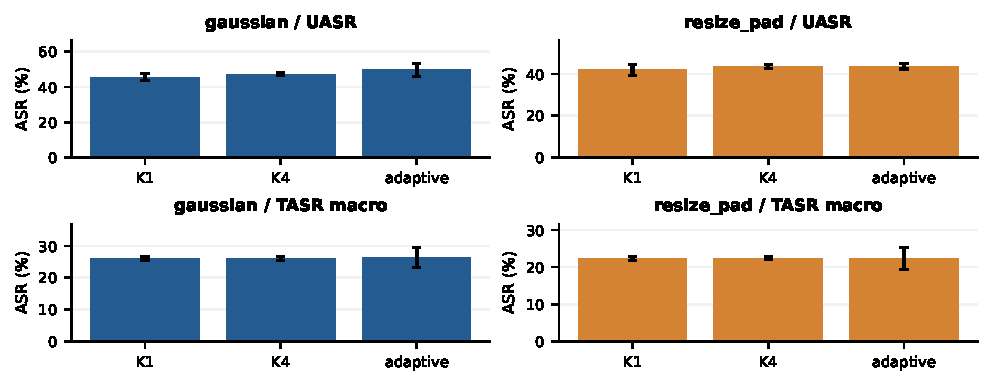
\includegraphics[width=\linewidth,height=2.45in,keepaspectratio]{images/D_main_report.pdf}
\caption{Side 7: K1 is the original nonadaptive attack; K4 is defense-unaware EOT matching; adaptive is defense-aware K4. Eligibility remains the undefended clean-correct set. Targeted panels equally average all ten targets. Both sizes appear in the effect table.}
\end{figure}

\begin{center}\small
\begin{tabular}{lrlr}\toprule
Defense & Side & Metric & Adaptive - unknown K4: pp [95\% CI]\\\midrule
gaussian & 5 & U & +1.38 [+1.29, +1.48]\\
gaussian & 5 & T macro & +1.70 [+1.66, +1.73]\\
resize/pad & 5 & U & +0.65 [+0.55, +0.77]\\
resize/pad & 5 & T macro & +1.31 [+1.28, +1.34]\\
gaussian & 7 & U & +2.41 [+2.21, +2.61]\\
gaussian & 7 & T macro & +0.27 [+0.23, +0.32]\\
resize/pad & 7 & U & -0.06 [-0.27, +0.15]\\
resize/pad & 7 & T macro & -0.11 [-0.16, -0.06]\\
\bottomrule\end{tabular}\end{center}
At side 7, adaptive-minus-unknown-K4 UASR is +2.41 pp for Gaussian blur and -0.06 pp for resize/pad. Defense awareness is therefore not uniformly stronger in this experiment. ASR alone cannot assign all defended errors to the patch; paired defense-only errors and net error/target-rate increases are archived alongside full clean/patched accuracy. Per-patch elapsed cost spans optimizer-function entry to artifact assembly; external model/data loading and final serialization are excluded.
Interactive graphics began sharing the GPU during later fixed-step D runs. Their observed runtimes do not isolate defense overhead; update/EOT budgets are unchanged. The C time-matched runs ended earlier.
\clearpage
\section*{D continued: attack strength and Monte Carlo stability}
Strength diagnostics are fixed at side 7, target 3 and the untargeted task, both defenses, and all three seeds. The two additional optimization conditions change one factor at a time: 2,000 updates with K=4, or 1,000 updates with K=8. These 24 patches remain separate from the 561 main optimizations. They test two prespecified objectives and are not substitutes for the full ten-target main matrix.


\begin{figure}[h]
\centering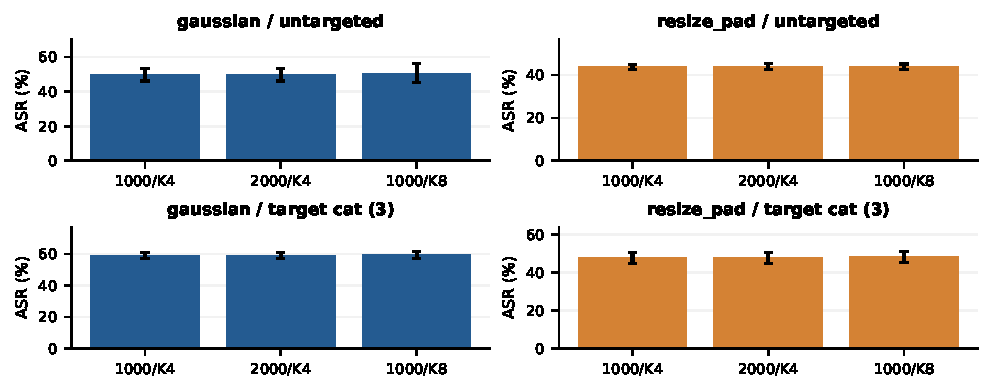
\includegraphics[width=\linewidth,height=2.5in,keepaspectratio]{images/D_strength_checks_main.pdf}
\caption{Prespecified strength checks: update budget and EOT count vary separately. Each bar shows mean ASR and sample standard deviation across the three patch seeds. Main settings are evaluated against the corresponding defense.}
\end{figure}

Across these four diagnostic tasks, doubling updates changes mean ASR by +0.006 to +0.108 pp; doubling K changes it by -0.015 to +0.803 pp. These small changes do not establish global convergence.
\begin{center}\small
\begin{tabular}{llrrr}\toprule
Defense & Task & 8 draws: ASR (\%) & 32 draws: ASR (\%) & Difference (pp)\\\midrule
gaussian & U & 49.657 & 49.554 & -0.103\\
gaussian & target 3 & 59.034 & 59.049 & +0.015\\
resize/pad & U & 43.709 & 43.571 & -0.138\\
resize/pad & target 3 & 47.571 & 47.607 & +0.036\\
\bottomrule\end{tabular}\end{center}
These are the same selected patches, with no further optimization. The first eight draws are shared with the 32-draw estimate. Additional draws reduce Monte Carlo noise, rather than providing additional independent images or a majority-vote defense.
\section*{A continued: denominators, pairing, and auditing}
For classifier $f$, let $S_f=\{i:f(x_i)=y_i\}$ and $S_{f,t}=\{i\in S_f:y_i\ne t\}$. UASR averages patched errors over $S_f$; TASR averages target hits over $S_{f,t}$. Patched accuracy instead uses all test images. Defenses retain the undefended classifier's fixed eligibility set. Each image has eight paired transform/defense draws; their outcomes are averaged before aggregation over images. Empty eligibility is undefined, never zero.

Three independently optimized patches provide mean and sample standard deviation (ddof=1). Targeted results first form an equal-weight ten-target macro average. Paired differences use the same image, draw, seed, and checkpoint. Confidence intervals resample whole images within true classes 2,000 times with seed 4242, retaining all draws and the fixed three patch seeds; target denominators are recomputed inside each bootstrap. They exclude classifier-training variability. SHA-256 checks, duplicate/missing-condition detection, exact official image sets, and raw-to-summary recomputation guard all 1,638 final files.
\clearpage
\section{Qualitative evidence, limitations, and conclusion}


\begin{figure}[h]
\centering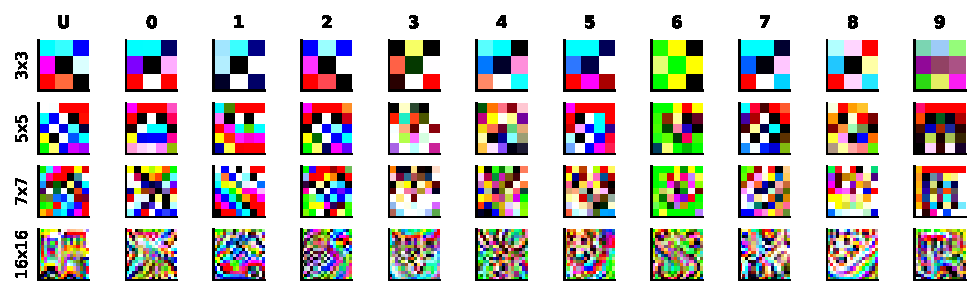
\includegraphics[width=\linewidth,height=1.85in,keepaspectratio]{images/B_patch_gallery_main.pdf}
\caption{Actual learned ResNet textures, seed 101. Rows are sides 3/5/7/16; columns are untargeted (U) and targets 0--9. These examples illustrate patterns, not an additional optimization or a semantic explanation.}
\end{figure}



\begin{figure}[h]
\centering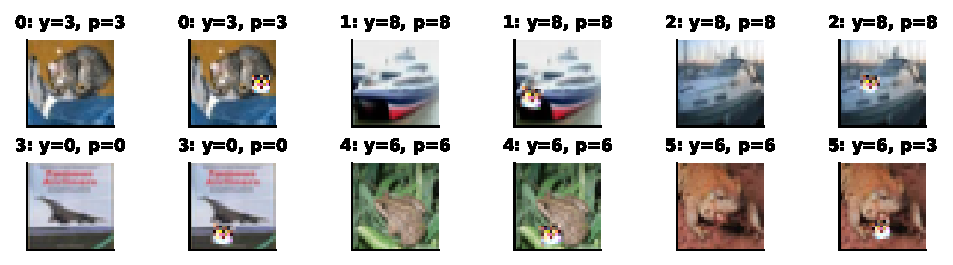
\includegraphics[width=\linewidth,height=1.65in,keepaspectratio]{images/B_fixed_examples_main.pdf}
\caption{First six IDs from the fixed qualitative list, draw 0, the 7-by-7 target-3 seed-101 patch. Each clean/patched pair shows true class y and prediction p. The full list of IDs 0--11, eligibility flags, and success/failure labels is in the supplement.}
\end{figure}

The fixed 12-image list contains 3 target hits and 7 misses among 10 eligible examples; 2 are excluded. Across the complete side-7 ResNet target matrix, target 5 has the highest mean TASR (62.21\%) and target 7 the lowest (3.83\%). The displayed target-3 texture has adjacent-pixel total variation 0.737 and 73.9\% of its non-DC energy at radial frequencies at least 0.25 cycles/pixel. These are descriptive observations, not causal feature attribution.
\paragraph{Interpretation and limits.}
The archived measurements support only the specified digital patch space, models, splits, and budgets. A 16-by-16 square covers 25\% nominal area, so learned-texture effects must be read alongside matched occlusion. Small patches may fail and target classes may differ; neither is removed from the report. Measured spectral energy and total variation are provided as descriptive texture statistics, without inferring which visual features cause a network's decision. Three patch repeats do not establish stability over independently trained classifiers. Attack failure is neither a certified robustness result nor evidence for physical printing/camera effectiveness. Held-out isolation constrains method selection but does not represent all architectures.

\paragraph{Responsibilities and AI assistance.}
The planned scope maps A (xy195) to data/models/metrics, B (yz1047) to shared patch optimization and base attacks, C (bz138) to transfer/ensembles/budgets, and D (zy232) to defenses/adaptation/strength checks. An AI coding assistant assisted implementation, execution, debugging, analysis, and writing. Numerical claims in this report are generated from archived measured records and validated by the included checks. This statement describes the workflow and planned responsibility mapping; it does not attest to unobserved individual effort or attendance.
\clearpage
\begin{thebibliography}{9}
\bibitem{brown} T. B. Brown et al. Adversarial Patch. arXiv:1712.09665, 2017. \url{https://arxiv.org/abs/1712.09665}.
\bibitem{athalye} A. Athalye, N. Carlini, and D. Wagner. Obfuscated Gradients Give a False Sense of Security. ICML, PMLR 80:274--283, 2018. \url{https://proceedings.mlr.press/v80/athalye18a.html}.
\bibitem{cifar} A. Krizhevsky. Learning Multiple Layers of Features from Tiny Images. Technical report, 2009. \url{https://cave.cs.toronto.edu/kriz/cifar.html}.
\bibitem{resnet} K. He et al. Deep Residual Learning for Image Recognition. CVPR, 2016. \url{https://arxiv.org/abs/1512.03385}.
\bibitem{vgg} K. Simonyan and A. Zisserman. Very Deep Convolutional Networks for Large-Scale Image Recognition. ICLR, 2015. \url{https://arxiv.org/abs/1409.1556}.
\bibitem{densenet} G. Huang et al. Densely Connected Convolutional Networks. CVPR, 2017. \url{https://arxiv.org/abs/1608.06993}.
\end{thebibliography}
\end{document}
